% outline

% title-me
% EBCWA problem
% ideal solution (solution attributes)
% DITA (verse fail http://media.boreme.com/post_media/2008/tank-toll.jpg)
% docutils (nearly success)
%  MS-Word -> docbookXML -> reST
%  recognise verses (1saiah)
%  verse role
%  biblepassage directive
%  document linking/sharing
%  draft-comment
% sphinx
%  conf.py
%  toctree
%  4 types (all html, 1 pdf, 1 epub, 1 google-docs) (bible-version, draft)
% paver
%  paver <type> book <version> <draft> <force>
%  override conf.py with cog
%  run pdflatex with rubber
%  singlehtml->insert css with cog->google-doc

\newcommand{\rst}{reStructuredText}
\documentclass{beamer}
\usepackage{minted}
\usetheme{default}
\hypersetup{colorlinks=true}
\usepackage{framed}
\usepackage[normalem]{ulem}

\title{TheoreST: Publishing Theology with Python}
\author{Carl Cerecke}
\institute{Evangelical Bible College of Western Australia}
\date{September 8, 2013}

\begin{document}

    \begin{frame}[plain]
        \titlepage
    \end{frame}

    \begin{frame}{Overview of the talk}
        \begin{itemize}
        \item Problem (and ideal solution)
        \item A tank is not the solution
        \item Proprietary format $\rightarrow$ \rst
        \item \rst $\rightarrow$ web/pdf/epub
            \begin{itemize}
            \item docutils
            \item sphinx
            \end{itemize}
        \item Automating with \texttt{paver}
        \item Other tools/technologies
        \item Todo\ldots
        \end{itemize}
    \end{frame}
    
    \begin{frame}{The problem}
        \begin{itemize}
        \item ~300 books in MS Word format (written over 20+ years)
            \begin{itemize}
            \item Systematic Theology
            \item Pastoral Theology
            \item Commentaries
            \item Miscellaneous topics 
            \end{itemize}
        \item Distribute as widely and conveniently as possible
        \item ``Freely you have been given, freely give''
        \end{itemize}
    \end{frame}
    
    \begin{frame}{The (ideal) solution}
        \begin{itemize}
        \item One authoritative source, multiple outputs
        \item Share common document fragments
        \item Bible version independent
        \item Bible references hyperlinked: \href{http://some.url}{John 3:16}
        \item Build individual books (pdf/epub), or whole collection (html)
    \end{itemize}
\end{frame}
    
\begin{frame}
    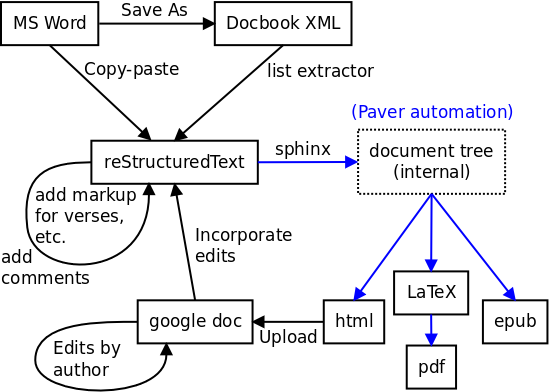
\includegraphics[keepaspectratio=true, width=\paperwidth]{theorest_process.png}
\end{frame}
    
    \begin{frame}{DITA: the Wrong Way}
        \begin{itemize}
        \item DITA: Enterprise-level technical documentation
        \item XML
        \item Java
        \item Deal-breaker: Too static.\\
            Dynamically determine bible-reference URLs during document creation?
        \end{itemize}
    \end{frame}
    
    \begin{frame}[plain]
        \centerline{
\includegraphics[keepaspectratio=true, width=\paperwidth]{tank-toll.jpg}}
    \end{frame}
    
    \begin{frame}{\rst markup language (PEP 287)}
        Put example here\\
        include roles and directives
    \end{frame}

    \begin{frame}{MS Word format to \rst}
        
\includegraphics[keepaspectratio=true, width=\paperwidth]{typewriter_keyboard.jpg}
    \end{frame}
    
    \begin{frame}{MS Word problems}
    No styles\\
        Enumerated lists
        \begin{framed} %{enumerated lists}
            \ldots\\
3. EVALUATION\\
\quad (a) Persecuted in Damascus; escapes in basket (Acts 9:20-25)\\
\quad (b) Driven out of Jerusalem, sent to Tarsus (Acts 9:28-30).\\
\quad (c) Stoned at Lystra and thought to have died (Acts 14:19).\\
        \quad (d) Paul whipped and imprisoned at Phillipi (Acts 16:16-24).\\
        \ldots
    \end{framed}
    Solution:\\
    \emph{Save As...} docbook XML format. Guess indent level.  
    \end{frame}
    
    \begin{frame}[fragile]
        \frametitle{Recognising bible references}
         Want to replace:\\
         \begin{verbatim}Lorem ipsum John 3:16 dolor
\end{verbatim}
         with:\\
         \begin{verbatim}Lorem ipsum `John 3:16` dolor
\end{verbatim}
Other examples:
\begin{itemize}
\item multiple verses: John 3:16,20
\item verse range: John 3:16-20
\item whole chapter: John 3
\item Multi chapter: John 3:16, 4:4
\item Multi book, chapter, verse, range:\\
    John 3:16-18,20,4:1, 3 John 1:2, Luke 1:1
\end{itemize}
\end{frame}

\begin{frame}{Regular expressions}
    
\includegraphics[keepaspectratio=true, width=0.9\paperwidth]{regular_expressions.png}

High-level view:
\begin{itemize}
\item A mini-language for specifying a set of strings.
\item An efficient \emph{recogniser} for that set of strings.
\end{itemize}

\end{frame}



\begin{frame}[fragile]
    
\begin{minted}{python}
names = ['Genesis', 'Exodus', ..., 'Revelation']
re_names = '('+'|'.join(names)+')'
re_raw = '('+re_names+r'\s+\d+:(\s*(,|-|;|:|'+\
    re_names+'|\d+))+'+')'
re_bibref = re.compile(re_raw)

def bibquote(text):
    return re_bibref.sub(r'`\1`', text)
\end{minted}

What about lsaiah? or I Corinthians? Argh!

\end{frame}

\begin{frame}[fragile]{Parsing the verse roles}
Need to translate `John 3:16-18,20` into:

\begin{minted}{html}
<a href="http://bible.xyz/ESV/john3+3:16-18">
John 3:16-18</a>,
<a href="http://bible.xyz/ESV/john3+3:20">20</a>
\end{minted}

Actually, internal document-tree nodes representing links.

\end{frame}

\begin{frame}[fragile]{Tokenisation}
Use python's own tokeniser

\begin{minted}{bash}
> echo "John 3:16-18,20" | python3 -m tokenize
1,0-1,4:            NAME           'John'         
1,5-1,6:            NUMBER         '3'            
1,6-1,7:            OP             ':'            
1,7-1,9:            NUMBER         '16'           
1,9-1,10:           OP             '-'            
1,10-1,12:          NUMBER         '18'           
1,12-1,13:          OP             ','            
1,13-1,15:          NUMBER         '20'           
1,15-1,16:          NEWLINE        '\n'           
2,0-2,0:            ENDMARKER      ''             
\end{minted}

\end{frame}

\begin{frame}[fragile]{Parsing}

\begin{itemize}
\item Plenty of parser-generators available.

\item Too heavyweight.

\item Verse references don't nest.

\item But do need lookahead:
\begin{minted}{python}
'John' '3' ':' '16' '-' '18' ',' '20' ...
\end{minted}

\item Solution: Use a state machine

\pause
\item Problem: No goto :-(

\pause
\item Solution: My goto function decorator:\\
\url{http://code.activestate.com/recipes/576944-the-goto-decorator/}

\pause
\item Problem: Only python 2
\end{itemize}
\end{frame}

\begin{frame}[fragile]{Parsing state machine}

One method per state.

Each method-state returns next method-state

\begin{minted}{python}
def parse(self):
    ...
    state = self.p_book            # start state
    while state:
        state = state()
		
def p_book(self):                  # expecting a book
    self.book = self.swallow(Book) # exception if not Book
    self.text += self.book.value   # collect link text
    return self.p_chapter          # 'goto' this state
	
def p_chapter(self):               # expecting a chapter
    ...
\end{minted}
\end{frame}

\begin{frame}{Adding verse role to sphinx}
\end{frame}

\begin{frame}{Adding biblepassage directive to sphinx}
\end{frame}

\begin{frame}{Automating the build process}
Problem: minimise effort to build documentation

What I want to build:
\begin{itemize}
\item All documents in integrated sphinx website
\item Individual documents as pdf/epub/html-for-google-docs
\end{itemize}
For each build I want to specify:
\begin{itemize}
\item bible version (ESV, KJV, NET, etc.)
\item include draft comments
\item possibly other options (e.g. force)
\end{itemize}
Also, minimal duplication in sphinx \texttt{conf.py}\\

Solution: paver

\end{frame}

\begin{frame}{Automating the build process with paver}
"Paver is a Python-based build/distribution/deployment 
scripting tool along the lines of Make"

Command line I want:
\begin{itemize}
\item \texttt{paver html} (integrated website with all books)
\item \texttt{paver pdf john} (pdf ouput of John, default bible version)
\item \texttt{paver epub john}
\item \texttt{paver pdf john NET draft} (use NET bible, show comments)
\item \texttt{paver single john} (html for upload to google-docs)
\item \texttt{paver pdf matthew mark luke john} (multiple books)
\end{itemize}

Sets up configuration, then calls \texttt{sphinx-build}

\end{frame}

\begin{frame}[fragile]{Sharing a single sphinx config file}

Project file hierarchy:

\begin{tabular}{|l|l|}
\hline
\texttt{/} & root directory \\
\texttt{/index.rst} & for integrated website with all books \\
\texttt{/conf.py} & symbolic link to \texttt{/src/conf.py}\\
\hline
\texttt{/src/} & All common configuration and code\\
\texttt{/src/conf.py} & Common sphinx configuration file\\
\hline
\texttt{/\emph{group}/\emph{book}/index.rst} & for stand-alone documents\\
\texttt{/\emph{group}/\emph{book}/conf.py} & symbolic link to \texttt{/src/conf.py}\\
\texttt{/../../conf\_override.py} & append to \texttt{conf.py}\\
\hline
\end{tabular}


\end{frame}

\begin{frame}[fragile]{Handling sphinx options?}

\begin{itemize}
\item Sphinx configuration file is python code.

\item Can override simple name=value options on command line:\\
\texttt{sphinx-build -Dbible\_version=ESV}

\item But complex overrides (i.e. python code) fail:
\sout{\texttt{-Dlatex\_elements['papersize']='a4paper'}}

\item Some overrides are static per-book:\\
Generated \LaTeX\ file = \texttt{john.tex}

\item Others are dynamic--- at generation time:
\texttt{paper\_type = "letter"}
\end{itemize}

Solution: code generation with \emph{cog}
\end{frame}

\begin{frame}[fragile]{Taming the sphinx config file with \emph{cog}}

\url{http://nedbatchelder.com/code/cog/}

\begin{itemize}
\item Use python code in a file to generate part of the file

\item At the end of sphinx config file:
\begin{minted}{python}
#[[[cog 
#include('conf_override.py')
#cog.out('\n')
#if 'override_text' in globals():
#    cog.out(override_text)
#]]]
#[[[end]]]
\end{minted}

\item Cog runs python code between \texttt{[[[cog} and \texttt{]]]}

\item Output (via \texttt{cog.out}) appears between \texttt{]]]} and \texttt{[[[end]]]}

\item In paver stdlib: \texttt{paver.doctools.cog(\emph{options})}
\end{itemize}
\end{frame}

\begin{frame}[fragile]{The draft-comment-edit cycle}
%\begin{enumerate}
%\item Document in draft form.
%\item Comments are made on that draft
%\item Changes are made based on comments.
%\end{enumerate}

Quote from one of the authors:

\begin{quote}
I come from a pre computer background which means I can write material and
send out emails plus do some limited scanning but nothing else
\end{quote}

Editing \rst\ source? I don't think so.

Current Solution:

\begin{itemize}
\item Publish to html.
\item Upload to google-drive, converting to google doc.
\item Author edits google doc.
\item I incorporate changes to \rst source.
\end{itemize}
Conversion is poor. Need way to programattically create google docs.
\end{frame}

\begin{frame}[fragile]{TheoreST technology overview}
\begin{itemize}
\item \url{https://github.com/cdjc/theoreST}
\item python 3.3
\item sphinx
\item paver (build tool)
\item cog (code generation tool)
\item \LaTeX\  and rubber (generating pdf)
\item Linux Mint 15 virtualbox VM
\item Wing IDE Professional (thanks nz pycon!)
\end{itemize}
\end{frame}

\begin{frame}{Future work}
\begin{itemize}
\item Continue converting documents to reST.
\item Robust versioning scheme.
\item Translation (with the aid of google-translate).
\item Dynamic bible-version selection on website.
\item Greek/Hebrew/Aramaic hyperlinks.
\item Website hosting.
\item Formatting tweaks.
\item Fix bugs. Add more tests.
\item Use more github features.
\end{itemize}

\end{frame}
\end{document}
